%%%%%%%%%%%%%%%%%%%%%%%%%%%%%%%%%%%%%%%%%%%%%%%%%%%%%%%%%%%%%%%%%%%%%%%%%%%%%%%
%%% Web Security 101 %%%%%%%%%%%%%%%%%%%%%%%%%%%%%%%%%%%%%%%%%%%%%%%%%%%%%%%%%%
%%%%%%%%%%%%%%%%%%%%%%%%%%%%%%%%%%%%%%%%%%%%%%%%%%%%%%%%%%%%%%%%%%%%%%%%%%%%%%%

\begin{frame}
    \frametitle{Finding Vulnerabilities in Web Applications}
    In a nutshell, \textbf{to find vulnerabilities in your web application}, ...
    \begin{enumerate}
        \item ... test various values for parameters used by the web application and see what happens (conceptually similar to fuzzing)
        \item ... check web application code for bugs that may lead to security vulnerabilities (typically missing checks of input values or missing countermeasures against certain types of attacks)
    \end{enumerate}
\end{frame}

\begin{frame}
    %\frametitle{OWASP TOP 10}

    The \href{https://owasp.org/www-project-top-ten/}{Open Web Application Security Project (OWASP)} maintains a list of Top 10 vulnerabilities in web applications.

    \begin{center}
        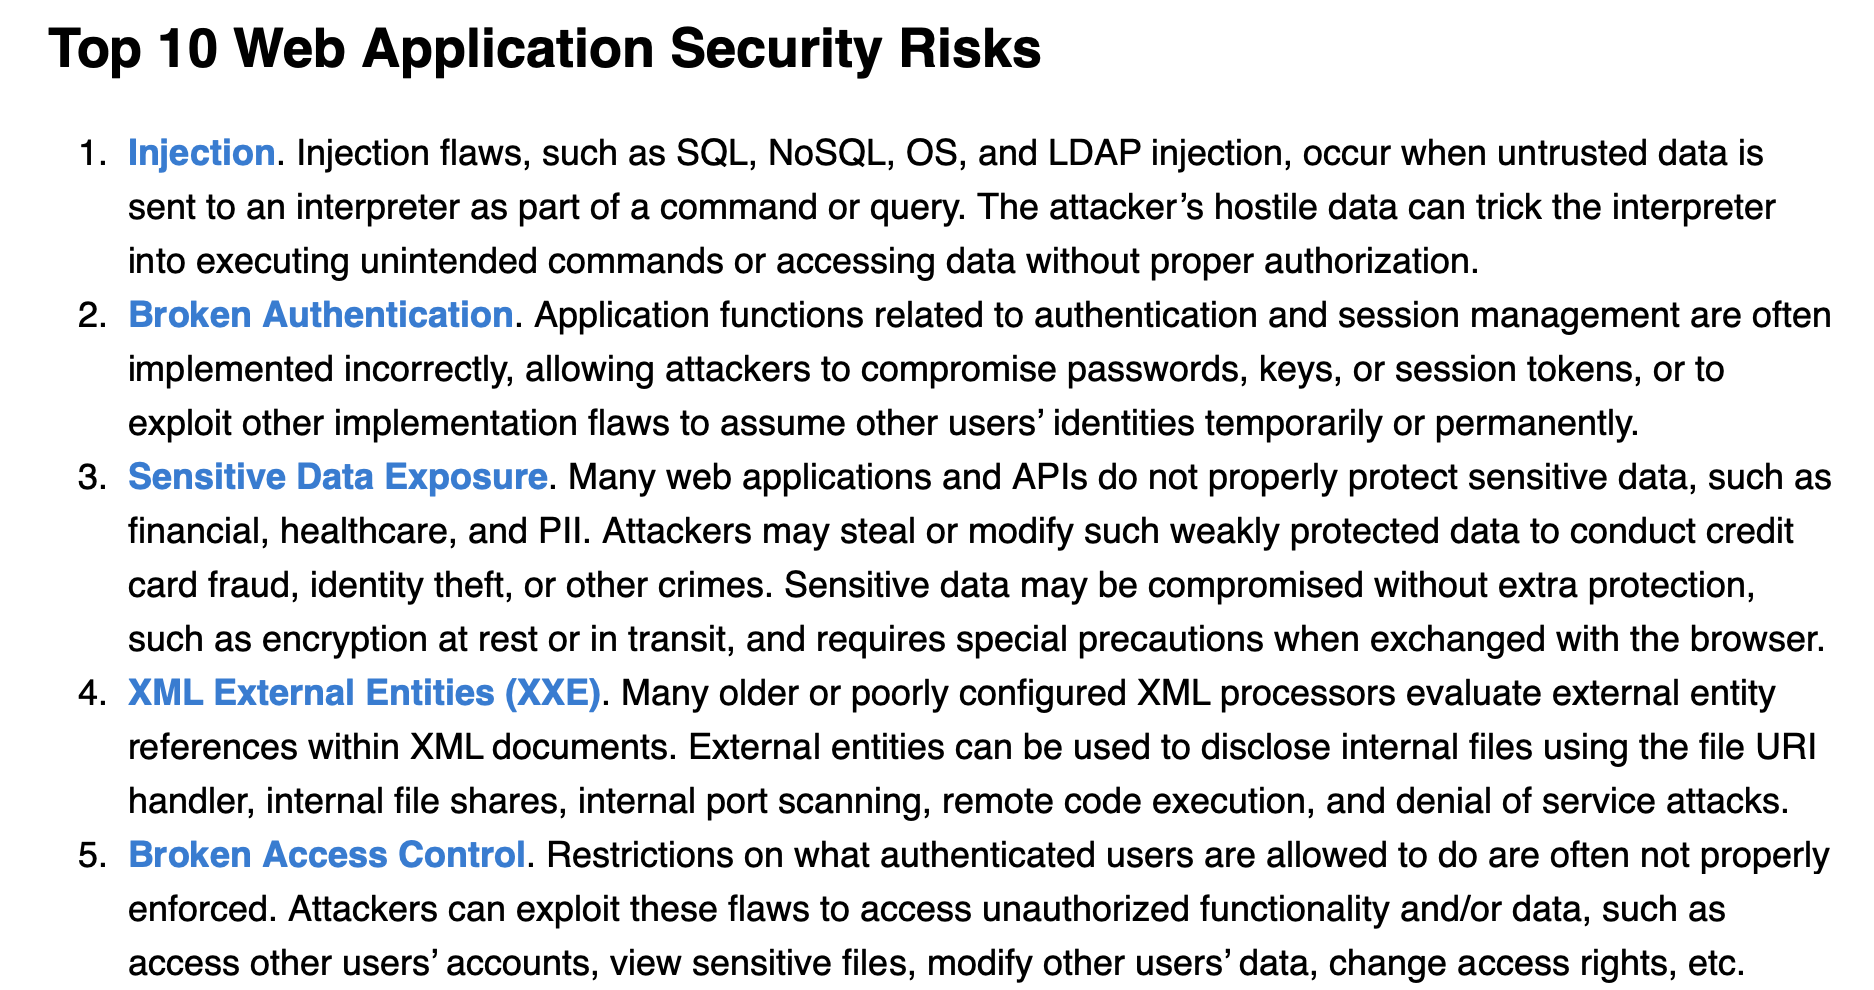
\includegraphics[scale=.35,angle=2]{img/owasp-top10.png}    
    \end{center}
\end{frame}

%%%%%%%%%%%%%%%%%%%%%%%%%%%%%%%%%%%%%%%%%%%%%%%%%%%%%%%%%%%%%%%%%%%%%%%%%%%%%%%
%%% Naming Conventions %%%%%%%%%%%%%%%%%%%%%%%%%%%%%%%%%%%%%%%%%%
%%%%%%%%%%%%%%%%%%%%%%%%%%%%%%%%%%%%%%%%%%%%%%%%%%%%%%%%%%%%%%%%%%%%%%%%%%%%%%%

\begin{frame}
	\frametitle{Conventions}
	\begin{itemize}
		\item Alice, Bob: legitimate users
		\item Eve: malicious user, attacker
		\item Server: web server running a web application
		\item Client: web browser (or computer running the web browser)
	\end{itemize}
\end{frame}

%%%%%%%%%%%%%%%%%%%%%%%%%%%%%%%%%%%%%%%%%%%%%%%%%%%%%%%%%%%%%%%%%%%%%%%%%%%%%%%
%%% Setting Up Docker Containers %%%%%%%%%%%%%%%%%%%%%%%%%%%%%%%%%%%%%%%%%%%%%%
%%%%%%%%%%%%%%%%%%%%%%%%%%%%%%%%%%%%%%%%%%%%%%%%%%%%%%%%%%%%%%%%%%%%%%%%%%%%%%%

\begin{frame}
	\frametitle{GitHub Repo}
	\begin{itemize}
		\item \url{https://github.com/duplys/youve-been-hacked}
		\item Dockerfile \& setup instructions
		\item Write-ups
		\item Code
	\end{itemize}
\end{frame}

\begin{frame}
	\frametitle{Building Docker Image}
	\begin{itemize}
		\item Running the demo web application in a Docker container is the easiest way to get started
		\item \texttt{Docker} dir contains \texttt{Dockerfile} for the vulnerable web application
		\item Build the container using \texttt{make build} or \texttt{docker-compose}
	\end{itemize}
		
\end{frame}

\begin{frame}[fragile]
	\frametitle{Starting Docker Containers}
	\begin{itemize}
		\item You'll need an empty directory \texttt{tmp} in the \texttt{Docker} dir
		\item In \texttt{Docker} dir, run \verb|$ docker-compose up|
	\end{itemize}
\end{frame}

\begin{frame}[fragile]
	\frametitle{Setting up ZAP}
	You need to activate ZAProxy (ZAP), configure your browser to proxy via ZAP and import the public ZAP Root certificate (see \url{https://www.zaproxy.org/docs/docker/webswing/} for details). Do the following steps:
	\begin{itemize}
		\item Go to \verb|http://127.0.0.1:8080/zap/|
		\item You'll see how the ZAP Web UI starts
		\item Start a ZAP session, choose "don't want to persist"
		\item Select "Update All" in the "Manage Add-ons" window
	\end{itemize}
\end{frame}

\begin{frame}
	\frametitle{Setting up ZAP}
	\centering
	\includegraphics[scale=.2]{img/zap-new-session-find-ip-address-and-port-for-proxy.png}
\end{frame}

\begin{frame}
	\frametitle{Setting up ZAP}
	\begin{itemize}
		\item Go to "Tools" $\rightarrow$ "Options" $\rightarrow$ "Dynamic SSL Certificates" $\rightarrow$ "Save"
		\item Save ZAP certificate on your host and import it into your browser.
		\item Read off the ZAP's IP address and port number at the bottom of ZAP's window
		\item Configure your web browser to use that IP/port as proxy
	\end{itemize}
\end{frame}

\begin{frame}[fragile]
	\frametitle{Accessing the Vulnerable Web App through ZAP}
	\begin{itemize}
		\item Look up the vulnerable app container IP address (for \texttt{docker-compose})
		\item Run \verb|docker container inspect docker_vulnapp_1| and look for \verb|IPAddress:| under \verb|Networks:|
		\item If the container's IP address on your machine is \verb|x.y.z.w|, you can access the vulnerable web app under \verb|http://x.y.z.w/daten/kapitel1.html|
	\end{itemize}
\end{frame}

\begin{frame}[fragile]
	\frametitle{Cleaning Up}
	\begin{itemize}
		\item Run \verb|$ docker-compose down|
	\end{itemize}
\end{frame}